% Options for packages loaded elsewhere
\PassOptionsToPackage{unicode}{hyperref}
\PassOptionsToPackage{hyphens}{url}
\PassOptionsToPackage{dvipsnames,svgnames,x11names}{xcolor}
%
\documentclass[
  letterpaper,
  DIV=11,
  numbers=noendperiod]{scrreprt}

\usepackage{amsmath,amssymb}
\usepackage{iftex}
\ifPDFTeX
  \usepackage[T1]{fontenc}
  \usepackage[utf8]{inputenc}
  \usepackage{textcomp} % provide euro and other symbols
\else % if luatex or xetex
  \usepackage{unicode-math}
  \defaultfontfeatures{Scale=MatchLowercase}
  \defaultfontfeatures[\rmfamily]{Ligatures=TeX,Scale=1}
\fi
\usepackage{lmodern}
\ifPDFTeX\else  
    % xetex/luatex font selection
    \setmainfont[]{Times New Roman}
\fi
% Use upquote if available, for straight quotes in verbatim environments
\IfFileExists{upquote.sty}{\usepackage{upquote}}{}
\IfFileExists{microtype.sty}{% use microtype if available
  \usepackage[]{microtype}
  \UseMicrotypeSet[protrusion]{basicmath} % disable protrusion for tt fonts
}{}
\makeatletter
\@ifundefined{KOMAClassName}{% if non-KOMA class
  \IfFileExists{parskip.sty}{%
    \usepackage{parskip}
  }{% else
    \setlength{\parindent}{0pt}
    \setlength{\parskip}{6pt plus 2pt minus 1pt}}
}{% if KOMA class
  \KOMAoptions{parskip=half}}
\makeatother
\usepackage{xcolor}
\setlength{\emergencystretch}{3em} % prevent overfull lines
\setcounter{secnumdepth}{5}
% Make \paragraph and \subparagraph free-standing
\makeatletter
\ifx\paragraph\undefined\else
  \let\oldparagraph\paragraph
  \renewcommand{\paragraph}{
    \@ifstar
      \xxxParagraphStar
      \xxxParagraphNoStar
  }
  \newcommand{\xxxParagraphStar}[1]{\oldparagraph*{#1}\mbox{}}
  \newcommand{\xxxParagraphNoStar}[1]{\oldparagraph{#1}\mbox{}}
\fi
\ifx\subparagraph\undefined\else
  \let\oldsubparagraph\subparagraph
  \renewcommand{\subparagraph}{
    \@ifstar
      \xxxSubParagraphStar
      \xxxSubParagraphNoStar
  }
  \newcommand{\xxxSubParagraphStar}[1]{\oldsubparagraph*{#1}\mbox{}}
  \newcommand{\xxxSubParagraphNoStar}[1]{\oldsubparagraph{#1}\mbox{}}
\fi
\makeatother


\providecommand{\tightlist}{%
  \setlength{\itemsep}{0pt}\setlength{\parskip}{0pt}}\usepackage{longtable,booktabs,array}
\usepackage{calc} % for calculating minipage widths
% Correct order of tables after \paragraph or \subparagraph
\usepackage{etoolbox}
\makeatletter
\patchcmd\longtable{\par}{\if@noskipsec\mbox{}\fi\par}{}{}
\makeatother
% Allow footnotes in longtable head/foot
\IfFileExists{footnotehyper.sty}{\usepackage{footnotehyper}}{\usepackage{footnote}}
\makesavenoteenv{longtable}
\usepackage{graphicx}
\makeatletter
\def\maxwidth{\ifdim\Gin@nat@width>\linewidth\linewidth\else\Gin@nat@width\fi}
\def\maxheight{\ifdim\Gin@nat@height>\textheight\textheight\else\Gin@nat@height\fi}
\makeatother
% Scale images if necessary, so that they will not overflow the page
% margins by default, and it is still possible to overwrite the defaults
% using explicit options in \includegraphics[width, height, ...]{}
\setkeys{Gin}{width=\maxwidth,height=\maxheight,keepaspectratio}
% Set default figure placement to htbp
\makeatletter
\def\fps@figure{htbp}
\makeatother
% definitions for citeproc citations
\NewDocumentCommand\citeproctext{}{}
\NewDocumentCommand\citeproc{mm}{%
  \begingroup\def\citeproctext{#2}\cite{#1}\endgroup}
\makeatletter
 % allow citations to break across lines
 \let\@cite@ofmt\@firstofone
 % avoid brackets around text for \cite:
 \def\@biblabel#1{}
 \def\@cite#1#2{{#1\if@tempswa , #2\fi}}
\makeatother
\newlength{\cslhangindent}
\setlength{\cslhangindent}{1.5em}
\newlength{\csllabelwidth}
\setlength{\csllabelwidth}{3em}
\newenvironment{CSLReferences}[2] % #1 hanging-indent, #2 entry-spacing
 {\begin{list}{}{%
  \setlength{\itemindent}{0pt}
  \setlength{\leftmargin}{0pt}
  \setlength{\parsep}{0pt}
  % turn on hanging indent if param 1 is 1
  \ifodd #1
   \setlength{\leftmargin}{\cslhangindent}
   \setlength{\itemindent}{-1\cslhangindent}
  \fi
  % set entry spacing
  \setlength{\itemsep}{#2\baselineskip}}}
 {\end{list}}
\usepackage{calc}
\newcommand{\CSLBlock}[1]{\hfill\break\parbox[t]{\linewidth}{\strut\ignorespaces#1\strut}}
\newcommand{\CSLLeftMargin}[1]{\parbox[t]{\csllabelwidth}{\strut#1\strut}}
\newcommand{\CSLRightInline}[1]{\parbox[t]{\linewidth - \csllabelwidth}{\strut#1\strut}}
\newcommand{\CSLIndent}[1]{\hspace{\cslhangindent}#1}

\usepackage{booktabs}
\usepackage{longtable}
\usepackage{array}
\usepackage{multirow}
\usepackage{wrapfig}
\usepackage{float}
\usepackage{colortbl}
\usepackage{pdflscape}
\usepackage{tabu}
\usepackage{threeparttable}
\usepackage{threeparttablex}
\usepackage[normalem]{ulem}
\usepackage{makecell}
\usepackage{xcolor}
\usepackage{caption}
\usepackage{anyfontsize}
\usepackage{amsmath}
\usepackage{float}
\usepackage{pdflscape}
\usepackage{afterpage}
\usepackage{longtable}
\usepackage[table]{xcolor}
\usepackage{longtable}
\usepackage{booktabs}
\KOMAoption{captions}{tableheading}
\makeatletter
\@ifpackageloaded{bookmark}{}{\usepackage{bookmark}}
\makeatother
\makeatletter
\@ifpackageloaded{caption}{}{\usepackage{caption}}
\AtBeginDocument{%
\ifdefined\contentsname
  \renewcommand*\contentsname{Table of contents}
\else
  \newcommand\contentsname{Table of contents}
\fi
\ifdefined\listfigurename
  \renewcommand*\listfigurename{List of Figures}
\else
  \newcommand\listfigurename{List of Figures}
\fi
\ifdefined\listtablename
  \renewcommand*\listtablename{List of Tables}
\else
  \newcommand\listtablename{List of Tables}
\fi
\ifdefined\figurename
  \renewcommand*\figurename{Figure}
\else
  \newcommand\figurename{Figure}
\fi
\ifdefined\tablename
  \renewcommand*\tablename{Table}
\else
  \newcommand\tablename{Table}
\fi
}
\@ifpackageloaded{float}{}{\usepackage{float}}
\floatstyle{ruled}
\@ifundefined{c@chapter}{\newfloat{codelisting}{h}{lop}}{\newfloat{codelisting}{h}{lop}[chapter]}
\floatname{codelisting}{Listing}
\newcommand*\listoflistings{\listof{codelisting}{List of Listings}}
\makeatother
\makeatletter
\makeatother
\makeatletter
\@ifpackageloaded{caption}{}{\usepackage{caption}}
\@ifpackageloaded{subcaption}{}{\usepackage{subcaption}}
\makeatother

\ifLuaTeX
  \usepackage{selnolig}  % disable illegal ligatures
\fi
\usepackage{bookmark}

\IfFileExists{xurl.sty}{\usepackage{xurl}}{} % add URL line breaks if available
\urlstyle{same} % disable monospaced font for URLs
\hypersetup{
  pdftitle={Mappeeksamen IDR4000},
  pdfauthor={Kandidatnummer 512},
  colorlinks=true,
  linkcolor={blue},
  filecolor={Maroon},
  citecolor={Blue},
  urlcolor={Blue},
  pdfcreator={LaTeX via pandoc}}


\title{Mappeeksamen IDR4000}
\author{Kandidatnummer 512}
\date{2024-09-10}

\begin{document}
\maketitle

\renewcommand*\contentsname{Table of contents}
{
\hypersetup{linkcolor=}
\setcounter{tocdepth}{2}
\tableofcontents
}

\bookmarksetup{startatroot}

\chapter*{Introduksjon}\label{introduksjon}
\addcontentsline{toc}{chapter}{Introduksjon}

\markboth{Introduksjon}{Introduksjon}

Mappeeksamen i IDR 4000 består både av oppgaver gjort i gruppe men også
selvstendig arbeid.

Link til git: https://github.com/hennieengebretsen/Mappeeksamen

\bookmarksetup{startatroot}

\chapter{Assignment 1: Reliability and tools for reproducible data
science}\label{assignment1}

\section{Introduksjon}\label{introduksjon-1}

Reliabilitet er en utrolig viktig faktor innenfor fysiologisk testing.
Hvis man ønsker å følge utviklingen til en utøver over en lenger periode
er det viktig at testen vi benytter oss av, og utstyret som brukes i
testen måler tilnærmet likt hver gang. Hvis testene som blir brukt har
høy reliabilitet kan utøvere og trenere stole på at forskjellene i
resultater mellom ulike tester skyldes endringer i fysiologiske faktorer
og at det ikke er feilmålinger som gir utslag.

For å i ettertid kunne evaluere effekten av en treningsplan,
intervensjon eller periode må man kunne stole på testene som blir
gjennomført. Dersom testene som blir benyttet har lav reliabilitet, kan
det være vanskelig å skille mellom virkelige prestasjonsforbedringer og
tilfeldige variasjoner som skyldes unøyaktighet i målingene. Dette kan
resultere i at man endrer et godt fungerende treningsopplegg, eller at
man fortsetter med et dårlig fungerende treningsopplegg.

I idrettsvitenskapen forskes det gjerne på effekt av ulike
intervensjoner. Uavhengig av om det gjøres forskning på utrente eller
elite-utøvere er det viktig at målingene har høy reliabilitet. Dette med
bakgrunn i at vi vil levere god kvalitet i forskningen og at det skal
være litteratur man skal kunne stole på.

Det ble gjennomført fire testdager 28.08.2024, 29.08.2024, 9.09.2024 og
11.09.2024 for å teste \(\dot{V}O_{2maks}\). Formålet med disse testene
var å øve på å kunne gjennomføre fysiologiske tester med høy
reliabilitet. Reliabilitet refererer til graden av konsistens eller
pålitelighet i målinger evnen til å kunne reprodusere (W. G. Hopkins
2000), et eksempel på dette er ved fysiologisk testing som repeteres i
forskningsprosjekter, der bedre reliabilitet vil indikere hvor god
presisjonen er og måling av endring over tid (W. G. Hopkins 2000). Det
er mange begreper som er relevante for å kunne si noe om reliabilitet,
men standardavviket er et av disse. Standardavviket sier noe om hvor
langt unna verdiens gjennomsnittlige avstand er fra gjennomsnittet
(Spiegelhalter 2020).

Kroppens maksimale oksygenopptak (\(\dot{V}O_{2maks}\)) sier noe om
kroppens maksimale evne til å ta opp og omsette oksygen (Bassett and
Howley 2000). \(\dot{V}O_{2maks}\) kan beskrives ved hjelp av Ficks
likning: \(\dot{V}O_{2maks}\)=MVmaks x a-vO2differansemaks.
\(\dot{V}O_{2maks}\) måles ved at man måler hvor mye oksygen kroppen
klarer å omsette pr minutt . Det finnes ulike måter og fremstille
\(\dot{V}O_{2maks}\) på, de to av disse er absolutt \(\dot{V}O_{2maks}\)
beskrevet som (ml ×min-1) eller relative tall relatert til kroppsvekt
(ml/kg/min).

I resultatdelen har vi valgt å bruke relativ \(\dot{V}O_{2maks}\) for å
beregne reliabiliteten til testene vi har gjennomført. Vi har også valgt
å se på sammenhengen mellom relativ \(\dot{V}O_{2maks}\) og wattmaks
under \(\dot{V}O_{2maks}\)-testen. Forskning viser at høy
\(\dot{V}O_{2maks}\), sammen med god mekanisk effektivitet og høy
laktatterskel gir bedre utholdenhetsprestasjoner, noe som reflekteres i
høyere Wmaks/kg (Joyner and Coyle 2008).

\section{Metode}\label{metode}

\(\dot{V}O_{2maks}\)-testen ble gjennomført på en ergometersykkel med
bukkestyre (Lode Excalibur Sport; Lode B.V., Groningen, Nederland).
Kranken kalibreres på Lode-sykkelen før hver teststart. Dette gjøres for
å få nøyaktige tråkkdata på hver forsøksperson. Sykkel stilles inn etter
utøvers ønske for å sikre best mulig sittestilling ved første test.
Sykkel stilles inn etter nøyaktig samme mål ved senere tester for å
gjøre reliabiliteten høy. For å måle det maksimale oksygenopptaket ble
det brukt Vyntus (Jaeger Vyntus CPX, Hoechberg, Tyskland).
Gassanalysator kalibreres til \textless{} 2,0\% differanse og luftvolum
kalibreres til \textless{} 0,2\% differanse. Syklistene veies med de
klærne de skal sykle med, og 0,3kg trekkes fra (300g er et estimat på
vekten av klærne forsøkspersonen har på). For å kunne sikre god
relabilitet ble det tydeliggjort at man skulle replisere det siste
måltidet før test, ha det samme koffeininntaket, avstå fra alkohol og
tobakk de siste 72 timene før test og prøve å få tilnærmet lik søvn,
samt trene det samme dagen før test. Da dette er faktorer som kan spille
inn på prestasjon og metabolismen (Tanner and Gore 2012) og dermed
påvirke relabiliteten.

\(\dot{V}O_{2maks}\)-testen gjennomføres etter en fem minutters
standardisert oppvarming på ergometersykkelen. Oppvarmingen starter to
minutter på 11-12 i Borg, deretter to minutter på 15 i Borg før ett
minutt på 11-12 Borg. Testen starter på en belastning (Watt) basert på
deltagerens nivå i samråd med utøver og testleder. Det viktigste er at
påfølgende \(\dot{V}O_{2maks}\) tester starter på samme watt.
Wattbelastningen økte med 20W eller 25W (20W for kvinne og 25W for mann)
hvert minutt frem til utøveren når maksimal utmattelse. Maksimal
utmattelse ble i denne sammenheng ikke evne til å kunne opprettholde RPM
\textgreater{} 60. Under \(\dot{V}O_{2maks}\) var RPM valgfritt.
Testleder gjør verbal oppmuntring og sekundering underveis i testen. For
at verbal oppmuntring og instruksjon ved test skulle være lik etterstreb
vi å ha samme testleder til samme forsøksperson (Halperin, Pyne, and
Martin 2015). Det blir registrert nye oksygenmålinger hvert 30 sek, og
de to høyeste påfølgende målingene blir definert som
\(\dot{V}O_{2maks}\). Umiddelbart etter test oppgir utøveren opplevd
anstrengelse på Borg skala. Maks hjertefrekvens blir lest av fra utøvers
pulsklokke. Blodprøve ble tatt fra utøverens fingertupp 1 min etter endt
test for å måle {[}BLa-{]}. {[}BLa-{]} blir deretter målt ved hjelp av
en Biosen C-line (Biosen C-line Lactate Analyzer, EKF Diagnostic GmbH,
Barleben, Germany). Etter endt test ble det hentet ut data som videre
ble plottet inn i Excel og videre ført statistikk på ved hjelp av
Rstudio.

\section{Resultat}\label{resultat}

Etter at testene er gjennomført kan vi se nærmere på hver forsøkperson
sine data. Dette gir muligheten til å se på hver enkelt forsøksperson om
man finner dette interessant (Table 1.1). Verdiene man kan se i
tabellen, er verdier som er plottet etter endt
\(\dot{V}O_{2maks}\)-test.

\begin{table}[H]
\centering\begingroup\fontsize{6}{8}\selectfont

\begin{tabular}{l>{\raggedright\arraybackslash}p{0.5cm}>{\raggedright\arraybackslash}p{0.5cm}>{\raggedright\arraybackslash}p{0.5cm}>{\raggedright\arraybackslash}p{0.5cm}>{\raggedright\arraybackslash}p{0.5cm}>{\raggedright\arraybackslash}p{0.5cm}>{\raggedright\arraybackslash}p{0.5cm}>{\raggedright\arraybackslash}p{0.5cm}>{\raggedright\arraybackslash}p{0.5cm}>{\raggedright\arraybackslash}p{0.5cm}>{\raggedright\arraybackslash}p{0.5cm}>{\raggedright\arraybackslash}p{0.5cm}>{\raggedright\arraybackslash}p{0.5cm}>{\raggedright\arraybackslash}p{0.5cm}>{\raggedright\arraybackslash}p{0.5cm}>{\raggedright\arraybackslash}p{0.5cm}}
\toprule
\textbf{Parameter} & \textbf{1} & \textbf{2} & \textbf{3} & \textbf{4} & \textbf{5} & \textbf{6} & \textbf{7} & \textbf{8} & \textbf{9} & \textbf{10} & \textbf{11} & \textbf{12} & \textbf{13} & \textbf{14} & \textbf{15} & \textbf{16}\\
\midrule
Borg$_{max}$ & 19.2 (0.96) & 19 (0.82) & 18 (1.2) & 19 (0) & 19.5 (0.71) & 19 (0) & 17.5 (1.7) & 17 (NA) & 19.7 (0.58) & 20 (0) & 17.5 (0.71) & 18 (1.7) & 18.3 (0.58) & 18.8 (0.5) & 17 (1) & 19.5 (0.71)\\
VO$_{2max}$ (ml/kg/min) & 33.5 (1.5) & 43.7 (2.6) & 51.6 (4.1) & 37.1 (1.1) & 58.9 (0.64) & 45.5 (0.2) & 61.8 (1.9) & 43.5 (NA) & 58.8 (0.59) & 43.2 (0.89) & 56.5 (0.94) & 61.7 (3.1) & 51.3 (0.88) & 65.7 (1.1) & 39.8 (2.6) & 60.2 (1.2)\\
Watt/kg & 2.5 (0.14) & 3.58 (0.044) & 3.6 (0.46) & 3 (0.2) & 5.18 (0.082) & 3.51 (0.1) & 5.24 (0.2) & 3.93 (NA) & 4.92 (0.038) & 3.76 (0.014) & 4.93 (0.049) & 5.6 (0.4) & 3.87 (0.062) & 5.51 (0.1) & 2.85 (0.12) & 4.63 (0.065)\\
VO$_{2max}$ (ml/min) & 3240 (150) & 2700 (160) & 4130 (300) & 2860 (52) & 4390 (48) & 3710 (6.4) & 5130 (140) & 2540 (NA) & 4650 (41) & 3100 (64) & 3640 (97) & 4480 (230) & 4590 (48) & 4520 (59) & 4100 (270) & 4960 (130)\\
Watt$_{max}$ & 243 (13) & 221 (2.8) & 288 (36) & 231 (13) & 387 (6.1) & 286 (7.5) & 435 (19) & 230 (NA) & 389 (2.1) & 269 (1.2) & 318 (0) & 407 (29) & 347 (6.9) & 380 (5.7) & 293 (12) & 382 (3.1)\\
\bottomrule
\multicolumn{17}{l}{\textsuperscript{} Table 1.1: Tabellen viser hver deltakers gjennomsnitt og standardavvik i () på verdier vi har undersøkt}\\
\end{tabular}
\endgroup{}
\end{table}

Etter å ha gjennomført VO\textsubscript{2maks}-testene ser vi at
kvinnene på 1MAIDR har et gjennomsnittlig oksygenopptak på 3163 ± 484.
Mennene har derimot et gjennomsnittlig oksygenopptak på 4380 ± 515.

Reliabiliteten mellom t1 og t2 er 2.47\%, mens reliabiliteten mellom t3
og t4 er 4.78\%.

\subsection{Korrelasjon mellom Vo2maks og Wattmaks per
kg}\label{korrelasjon-mellom-vo2maks-og-wattmaks-per-kg}

\begin{figure}[H]

{\centering 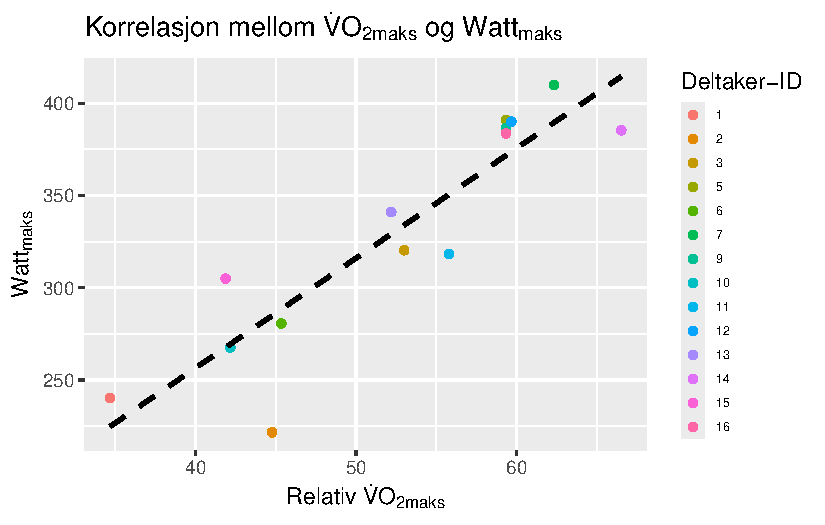
\includegraphics{01-reliability-tools_files/figure-pdf/unnamed-chunk-10-1.pdf}

}

\caption{Figur 1: Hvert punkt = én observasjon}

\end{figure}%

\section{Diskusjon}\label{diskusjon}

På bakgrunn av resultatene vi har observert under testing av
\(\dot{V}O_{2maks}\), kan man slå fast at reliabiliteten til metoden vi
har brukt er ganske god. Resultatene tyder på at vi får målt det vi er
ute etter på en god måte, og det vil variere lite i måle-utstyret fra
gang til gang.

Dette sikrer at vi med ganske god sikkerhet, kan fastslå om et
treningsprogram fungerer, ved å gjøre repeterte tester, med
treningsperioder i mellom.

\bookmarksetup{startatroot}

\chapter{Assignment 2: Regression models, predicting from
data}\label{assignment2}

\section{Introduksjon}\label{introduksjon-2}

En regresjonsmodell er en modell som kvantifiserer forholdet mellom en
eller flere uavhengige variabler og en avhengig variabel. Innen medisin
er regresjon den analysemtoden som er hyppigst anvendt. Det finnes
forskjellige regresjonsmodeller. De vanligste er lineær regresjon,
polynominal regresjon og logistisk regresjon. Hva man har av datasett
vil bestemme hvilken regresjonsmodell som egner seg best å benytte
(\textbf{Pisica2022?}).

En lineær regresjonsmodell er en modell der en kan estimere verdien av
en avhengig variabel basert på verdien av andre kjente uavhengige
variabler (\textbf{Pisica2022?}). I en slik modell benyttes en rett
linje for å lage en modell som beskriver dataen. Følgende funksjon
benyttes for å skape det lineære plottet:

y\textsubscript{i} = b\textsubscript{0} +
b\textsubscript{1}x\textsubscript{i} + e\textsubscript{i}

der y\textsubscript{i} er den avhengige variabelen som kan estimeres ved
å benytte de uavhengige variablene b\textsubscript{1}x\textsubscript{i}
og b\textsubscript{0}. b\textsubscript{0} er skjæringspunktet til grafen
og b\textsubscript{1} er stigningstallet til grafen.

\section{Part 1 - Lactate thresholds}\label{part-1---lactate-thresholds}

\subsection{Metode}\label{metode-1}

Dataene ble organisert i et mer hensiktsmessig format (tidy data) for å
forenkle videre analyse og modellering. Deretter ble ulike
regresjonsmodeller anvendt for å representere dataene. Nye
skjæringspunkter ble tegnet opp for å illustrere treningsintensitet ved
forskjellige laktatnivåer.

\subsection{Resultat}\label{resultat-1}

\begin{figure}

\centering{

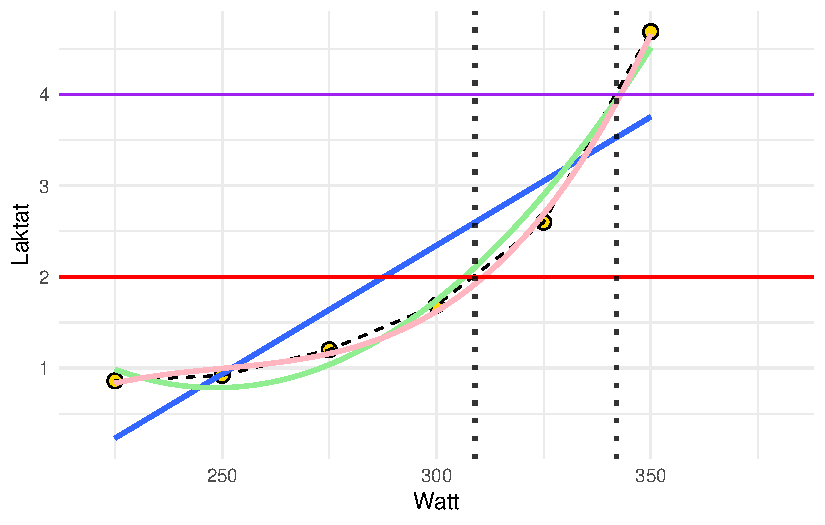
\includegraphics{02-regression-models_files/figure-pdf/fig-fig1-1.pdf}

}

\caption{\label{fig-fig1}Figur 1: Gule punkter = laktat og watt, blå
linje = lineær regresjon, grønn linje = andregradsligning, rosa =
tredjegradsligning.}

\end{figure}%

\subsection{Diskusjon}\label{diskusjon-1}

Vi har valgt å se på subject 10 fra datasettet Cyclingstudy. Vi gjør om
datasettet til tidydata. Dette gjør vi for å gi watt og laktat hver sine
verdier. Vi plotter inn laktatverdier og wattverdier (gule punkter).
Deretter tegner vi en stiplet linje som følger punktene. Vi gjør en
regresjonsanalyse, først en lineær modell (blå linje), deretter en
andregradsligning (grønn) og til slutt en tredjegradsligning (rosa).
Disse bruker vi for å observere hvilken modell som passer best i dette
tilfellet.

For å understreke hvor unøyaktig den lineære modellen er i dette
tilfellet, kan man på øyemål se at laktaten på 300W viser omtrent 2.4
mmol \textbf{×} L-1. Den faktiske laktaten på 300W er 1.69 mmol
\textbf{×} L-1 Figure~\ref{fig-fig1}.

\section{Part 2 - Predicting sizes of DNA
fragments}\label{part-2---predicting-sizes-of-dna-fragments}

\subsection{Metode}\label{metode-2}

For å predikere kalibreringskurven til qPCR, må en rekke prosesser på
molekylærlaboratoriet gjennomføres før dataene kan analyseres i R
Studio.

For å utføre en PCR på en 2\% agarosegel, ble det først tatt helblod fra
en forsøksperson for å ekstrahere DNA. Helblodet gjennomgikk ulike
prosesser hvor forskjellige løsninger og primere ble tilsatt. Dette
resulterte i et PCR-produkt. En elektroforese ble deretter kjørt for å
separere DNA-fragmentene fra PCR-reaksjonen. Etter fullført
elektroforese ble det tatt et bilde av 2\% agarosegelen.

Bildet fra elektroforesen ble analysert ved hjelp av ImageJ/Fiji, og
videre dataanalyser ble utført i R og R Studio. PCR-reaksjoners
effektivitet bestemmes av primerdesign og deres spesifisitet.

\subsection{Resultat}\label{resultat-2}

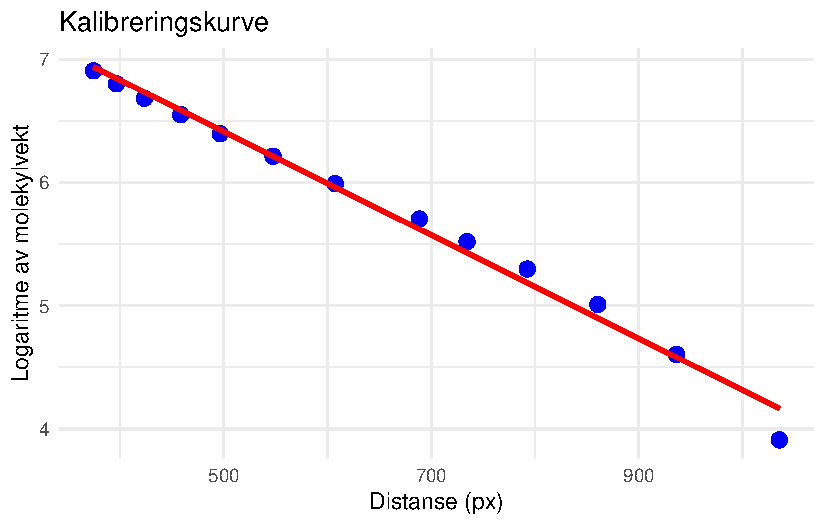
\includegraphics{02-regression-models_files/figure-pdf/unnamed-chunk-3-1.pdf}

\begingroup\fontsize{10}{12}\selectfont

\begin{longtable}[t]{>{}c>{}c>{}c}
\caption{Predikerte molekylvekter for ukjente distanser}\\
\toprule
\cellcolor[HTML]{404080}{\textcolor{white}{\textbf{Båndnummer}}} & \cellcolor[HTML]{404080}{\textcolor{white}{\textbf{Distanse (px)}}} & \cellcolor[HTML]{404080}{\textcolor{white}{\textbf{Predikert molekylvekt (bp)}}}\\
\midrule
\textbf{\cellcolor{gray!10}{1}} & \cellcolor[HTML]{F0F0FF}{\cellcolor{gray!10}{1208.5}} & \cellcolor[HTML]{F0F0FF}{\cellcolor{gray!10}{\cellcolor{red!25}31.22}}\\
\textbf{2} & \cellcolor[HTML]{F0F0FF}{600.5} & \cellcolor[HTML]{F0F0FF}{\cellcolor{yellow!25}400.05}\\
\textbf{\cellcolor{gray!10}{3}} & \cellcolor[HTML]{F0F0FF}{\cellcolor{gray!10}{18.5}} & \cellcolor[HTML]{F0F0FF}{\cellcolor{gray!10}{\cellcolor{green!25}4595.75}}\\
\textbf{4} & \cellcolor[HTML]{F0F0FF}{383.5} & \cellcolor[HTML]{F0F0FF}{\cellcolor{green!25}994.09}\\
\textbf{\cellcolor{gray!10}{5}} & \cellcolor[HTML]{F0F0FF}{\cellcolor{gray!10}{408.5}} & \cellcolor[HTML]{F0F0FF}{\cellcolor{gray!10}{\cellcolor{green!25}895.12}}\\
\addlinespace
\textbf{6} & \cellcolor[HTML]{F0F0FF}{436.5} & \cellcolor[HTML]{F0F0FF}{\cellcolor{green!25}795.93}\\
\textbf{\cellcolor{gray!10}{7}} & \cellcolor[HTML]{F0F0FF}{\cellcolor{gray!10}{470.5}} & \cellcolor[HTML]{F0F0FF}{\cellcolor{gray!10}{\cellcolor{green!25}690.14}}\\
\textbf{8} & \cellcolor[HTML]{F0F0FF}{508.5} & \cellcolor[HTML]{F0F0FF}{\cellcolor{green!25}588.45}\\
\textbf{\cellcolor{gray!10}{9}} & \cellcolor[HTML]{F0F0FF}{\cellcolor{gray!10}{559.5}} & \cellcolor[HTML]{F0F0FF}{\cellcolor{gray!10}{\cellcolor{yellow!25}475.12}}\\
\textbf{10} & \cellcolor[HTML]{F0F0FF}{618.5} & \cellcolor[HTML]{F0F0FF}{\cellcolor{yellow!25}370.95}\\
\addlinespace
\textbf{\cellcolor{gray!10}{11}} & \cellcolor[HTML]{F0F0FF}{\cellcolor{gray!10}{696.5}} & \cellcolor[HTML]{F0F0FF}{\cellcolor{gray!10}{\cellcolor{yellow!25}267.44}}\\
\textbf{12} & \cellcolor[HTML]{F0F0FF}{742.5} & \cellcolor[HTML]{F0F0FF}{\cellcolor{yellow!25}220.51}\\
\textbf{\cellcolor{gray!10}{13}} & \cellcolor[HTML]{F0F0FF}{\cellcolor{gray!10}{798.5}} & \cellcolor[HTML]{F0F0FF}{\cellcolor{gray!10}{\cellcolor{yellow!25}174.34}}\\
\textbf{14} & \cellcolor[HTML]{F0F0FF}{862.5} & \cellcolor[HTML]{F0F0FF}{\cellcolor{yellow!25}133.3}\\
\textbf{\cellcolor{gray!10}{15}} & \cellcolor[HTML]{F0F0FF}{\cellcolor{gray!10}{935.5}} & \cellcolor[HTML]{F0F0FF}{\cellcolor{gray!10}{\cellcolor{red!25}98.14}}\\
\addlinespace
\textbf{16} & \cellcolor[HTML]{F0F0FF}{993.5} & \cellcolor[HTML]{F0F0FF}{\cellcolor{red!25}76.94}\\
\bottomrule
\end{longtable}
\endgroup{}

\subsection{Diskusjon}\label{diskusjon-2}

\section{Part 3 - Interpreting a regression
table}\label{part-3---interpreting-a-regression-table}

\subsection{Metode}\label{metode-3}

\subsection{Resultat}\label{resultat-3}

\begin{figure}[H]

{\centering 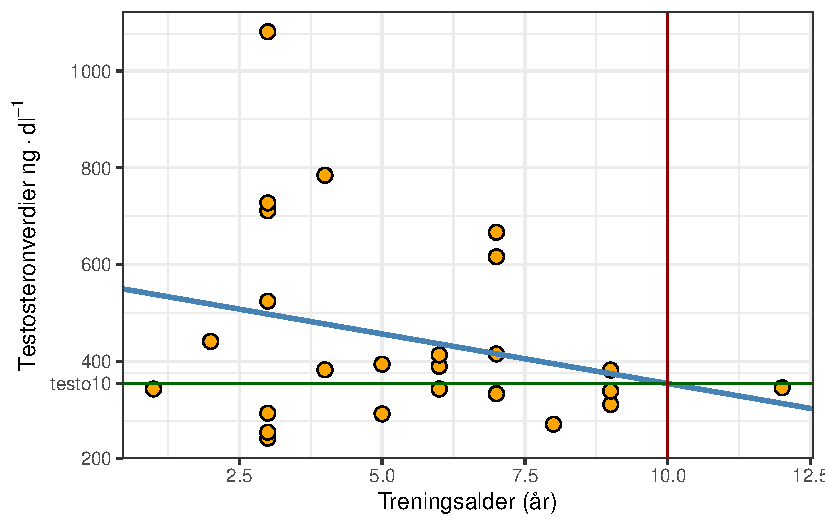
\includegraphics{02-regression-models_files/figure-pdf/tolkning av regresjonsmodell-1.pdf}

}

\caption{Figur 3: Sammenheng mellom treningsalder og testosteronverdier
i blodet}

\end{figure}%

\subsection{Diskusjon}\label{diskusjon-3}

Fra datasettet hypertrophy valgte vi å se på sammenhengen mellom
testosteronkonsentrasjon i blodet (ng \textbf{×} dl-1) og treningsalder
(antall år med trening). Den lineære modellen forteller at
testosteronkonsentrasjonen i blodet synker med 20.51 ng \textbf{×} dl-1
for hvert treningsår. Etter 10 år med trening, estimerer den lineære
modellen et testosteronnivå på 354.26 ng \textbf{×} dl-1.

Analysen av dataene viser en p-verdi på 0,1779, noe som indikerer at det
ikke er statistisk signifikant bevis for en sammenheng mellom
treningsalder og nivået av testosteron i blodet. Siden p-verdien er
høyere enn det vanlige signifikansnivået på 0,05, kan vi ikke avvise
nullhypotesen, som antyder at det ikke er noen betydelig effekt eller
sammenheng mellom de to variablene i dette datasettet. Dette betyr at
variasjonen i testosteronnivåer ikke ser ut til å være relatert til hvor
lenge individene har trent.

I analysen av sammenhengen mellom treningsalder og testosteronnivåer i
blodet ses det en t-verdi på 6.250. Den høye t-verdien på 6.250, og en
p-verdi på 0,1779. Denne p-verdien er høyere enn det vanlige
signifikansnivået på 0,05, noe som betyr at vi ikke har tilstrekkelig
statistisk bevis for å avvise nullhypotesen. Selv om t-verdien indikerer
en mulig sammenheng mellom treningsalder og testosteronnivå, er det ikke
nok evidens til å konkludere med at denne sammenhengen er signifikant.
Dermed kan vi konkludere med at selv om det kan være en tendens til en
sammenheng mellom treningsalder og testosteronnivåer, er resultatene fra
denne analysen ikke sterke nok til å si at treningsalder har en reell
effekt på testosteronnivåene i blodet.

\bookmarksetup{startatroot}

\chapter{Assignment 3: Drawing inference from statistical models, and
statistical power}\label{assignment3}

This assignment is set up as a statistical laboratory, we will perform
simulations and your assignment is to interpret and explain the results.
Create a report based on the code used in the lab and make sure you
answer the specified questions (1-8). You can be as creative as you want
and explore the results further.

\section{Spørsmål:}\label{spuxf8rsmuxe5l}

Et estimat representerer gjennomsnittet av det vi har målt i utvalget.
Det vil i lm1 og lm2 estimat gjennomsnitt på den ene variablen (y) i de
to ulike utvalgene.

SE (standard error) er standardfeilen vil være et mål på hvordan et
statistisk estimat til et utvalg kan variere fra populasjonen. For
modellen m1 er standard error 1.25 dette viser at det er noe usikkerhet
knyttet til et estimat av gjennomsnittet.

T-verdi kan ses på som en statistisk verdi hvor et forhold mellom
estimatet og standardfeilen.

\textbf{P-verdien} uttrykker sannsynligheten for å observere en
teststatistikk som er like ekstrem eller mer ekstrem enn det faktiske
resultatet, forutsatt at nullhypotesen (H₀) er sann. Den måler hvor godt
dataene samsvarer med nullhypotesen og bidrar til å vurdere usikkerheten
i resultatene. Lave p-verdier indikerer at resultatene sannsynligvis
ikke skyldes tilfeldigheter, og gir dermed støtte for å forkaste H₀.
Høye p-verdier tyder derimot på at resultatene kan forklares med
tilfeldigheter, og gir ikke tilstrekkelig grunnlag for å forkaste H₀.
Dermed fungerer p-verdien som et verktøy for å evaluere evidensen mot
nullhypotesen og trekke konklusjoner basert på statistiske analyser.

De to ulike modellene får ulike resultater en av grunnene til dette er
at det er ulikt utvalg i de to ulike modellene i lm1 er det n =8, mens i
lm2 er det n =40. Utvalgsstørrelsen vil ha en innvirkning på
resultatene, ved at man har et større utvalg vil den statistiske styrken
være høyere og det vil dermed være lettere å kunne oppdage om det vil
være en reell effekt en ser. Det samme vil gjelde for standardfeil ved
et større utvalg vil standardfeil til gjennomsnittet reduseres, en vil
da ha mindre konfidensintervall og estimatene vil kunne bli mer presist.

De mørke skyggeområdene til modellen viser de mer ``ekstreme''
tilfellene og jo lengre ut på de mørke områdene man kommer, vil de
resultatene være mindre sannsynlig å se.

\subsection{\texorpdfstring{Standard deviation of \textbf{estimate} and
avg. \textbf{se} for each
study.}{Standard deviation of estimate and avg. se for each study.}}\label{standard-deviation-of-estimate-and-avg.-se-for-each-study.}

Grunnen til at tallene er såpass like som de er for \textbf{SD} og
\textbf{avg se} er at begge beregningene er mål på variasjon. I denne
sammenhengen er standardfeilen et mål på hvor mye utvalgsgjennomsnittet
forventes å avvike fra det sanne populasjonsgjennomsnittet.

\subsection{P-value histogram}\label{p-value-histogram}

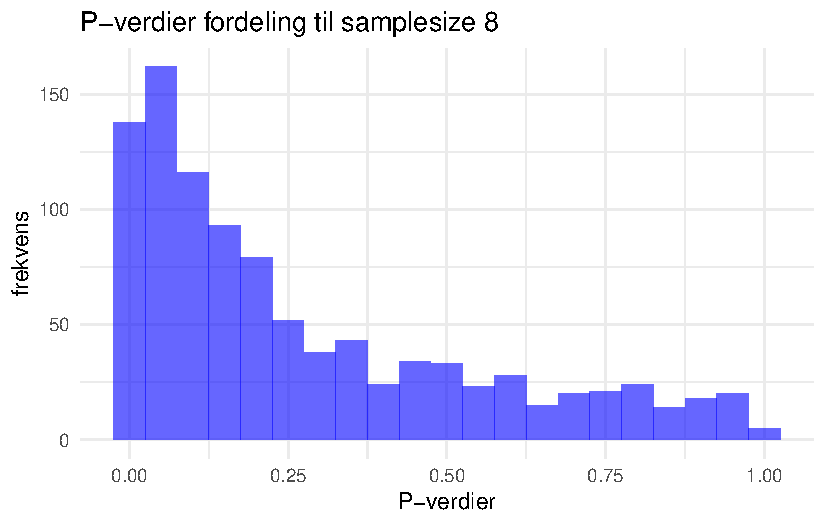
\includegraphics{03-statistical-inference_files/figure-pdf/P-verdi histogram SS8-1.pdf}

Histrogrammet for en utvalgstørrelse på 8, ser vi at det er et flertall
av obervasjoner med høye p-verdier. Dette henger sammen med lave
statistiske poweren og liten utvalgstørrelse

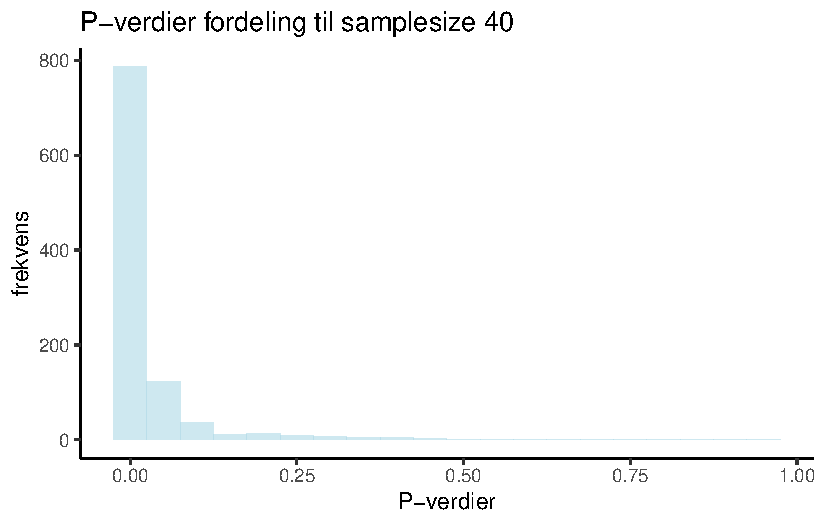
\includegraphics{03-statistical-inference_files/figure-pdf/P-verdi histogram SS40-1.pdf}

For et histogram med utvalgstørrelsen på 40 ses det at flere av
obervasjoene er sentrert mot lavere p-verdier. Dette fordi vi det er en
større utvalgstørrelse som gir en større statistik power

\subsection{Antall studier med statistisk
signifikans}\label{antall-studier-med-statistisk-signifikans}

Med utvalgsstørrelse på 8 ser vi at det er 227 studier som viser
statistisk signifikans, mens det ved utvalgsstørrelse på 40 er 865
studier som viser statistisk signifikans. Basert på dette som vi ser,
ser vi at det ved et støøre utvalg vil være flere signifikante resultat.
I denne situasjonen har jeg valgt å sette terskelen for signifikans til
\textless0.05

\subsection{Power of a one-sample
t-test}\label{power-of-a-one-sample-t-test}

Når vi gjør beregninger av utlvalgstørrelsene ser vi at utvlagstørrelsen
på 8 får en lavere statisitisk styrke (0.232) enn det vi får på en
utvalgstørrelse hvor vi har 40 (0.869). Et større utvalg gjør vil det
være høyere sannsynlighet for å kunne se den reelle effekten og at det
ikke bare er en tilfeldighet.

\subsection{Med signifikansnivå på 0.05 hvor mange studier gir ``falsk
positiv'' ved gjennomføring av mange repeterte
studier?}\label{med-signifikansnivuxe5-puxe5-0.05-hvor-mange-studier-gir-falsk-positiv-ved-gjennomfuxf8ring-av-mange-repeterte-studier}

Når det gjøres 1000 repeterte studier, vil det være 50 falske positive
om signifikansnivået er satt til 0.05. For utvalgstørrelsen på 8 fikk
jeg da 49 og for utvalgstørrelsen på 40 fikk en 59 falske positive Hvis
man velger å endre signifikansnivået til 0.025 vil en utlvalgstørrelse
på 8 gi endel færre falske positive med 30 mens for utvlagstørrelsen på
40 vil det være 22.

\bookmarksetup{startatroot}

\chapter{Assignment 4: Study designs}\label{assignment-4-study-designs}

\section{Introduksjon}\label{introduksjon-3}

Det vil i denne oppgave sammenlignes ulike studiedesign som tar for seg
den samme tematikken for å kunne se på hvorvidt ulike studier
presenterer og fremstiller sin forskning. Gode studiedesign sikrer god
og mer pålitelig forskning.

I denne oppgaven vil det ta for seg fem ulike studier som ser på
effekten av blokkperiodisering på det maksimale oksygenopptaket
(VO2maks) det har i studiene også blitt presentert andre funn, men disse
vil ikke bli diskutert inngående i denne oppgaven. Artiklene som er lagt
til grunn er (Bent R. Rønnestad, Øfsteng, and Ellefsen 2019; B. R.
Rønnestad et al. 2016, 2014; B. R. Rønnestad, Hansen, and Ellefsen 2014;
Breil et al. 2010) I de fem ulike artiklene er hensikten å finne ut
hvilken effekt blokkperiodisering (BP) verus tradisjonell periodisering
(TP) har på VO2max.~ Studiene er randomiserte kontrollerte forsøk (RCT).
I de ulike studiene har forskningsdeltagerne blitt inndelt i to ulike
grupper enten BP eller TP gruppen. Treningsvolumet innad i de to
gruppene var likt men periodiseringen i BP gruppen var annerledes da de
hadde mesosykluser med høy intensiv trening.

Studiene hadde mellom 16 til 22 deltagere de fleste studiene besto kun
av menn mens i andre studier var det både kvinner og menn (Breil et al.
2010) . Et fellestrekk for studiene var at det var godt trente
individer, hvor i noen av studiene var det utøvere på nasjonalt eller
internasjonalt nivå i konkurransesammenheng. To av studiene ser på
syklister mens for de tre andre ser den ene på hockeyspillere (Bent R.
Rønnestad, Øfsteng, and Ellefsen 2019) , en alpinister Breil et al.
(2010) og den sitse på langrennsløpere og skiskyttere B. R. Rønnestad et
al. (2016)

Intervensjonsvarigheten varierte imellom de ulike studiene
intervensjonen varierte fra 4-12 uker. Det ble i alle studiene
gjennomført testing pre og post intervensjonstart.

I de ulike studiene ble flere statistiske metoder benyttet for å
analysere dataene. Generelt ble gjennomsnitt ± standardavvik (SD)
rapportert for alle variabler, noe som gir en beskrivelse av både
sentralt mål og variasjon i dataene.

For å sammenligne baseline-målingene mellom gruppene, ble det i flere av
studiene benyttet en to-sidet unpaired t-test for uavhengige prøver.
Denne testen ble brukt for å vurdere om det var signifikante forskjeller
i variabler som VO2max, vekt og høyde ved starten av studiene. Videre
ble endringer mellom pre- og post-intervensjon i de samme gruppene
vurdert ved hjelp av to-sidet paired t-test som tester om det er
statistisk signifikante forskjeller i målingene innenfor hver gruppe.

For å vurdere effektene av intervensjonen på tvers av tid og gruppe,
benyttet flere av studiene to-veis ANOVA med repeterte målinger. Denne
metoden gjør det mulig å undersøke interaksjonseffekter mellom tid (pre-
vs.~post-intervensjon) og gruppe (f.eks., BP vs.~TP). Når ANOVA
resulterte i signifikante hoved- eller interaksjonseffekter, ble det
utført Tukey's HSD (Honestly Significant Difference) post-hoc tester or
å identifisere hvilke spesifikke grupper som skilte seg ut.

Effektstørrelse (ES) ble beregnet for å vurdere praktisk betydning av
forbedringer mellom gruppene. Cohen's d ble brukt til å beregne ES, og
kategoriseringen av ES fulgte standarden: 0.0--0.2 ble betraktet som
trivielt, 0.2--0.6 som lite, 0.6--1.2 som moderat, og verdier over 1.2
som store effekter William G. Hopkins et al. (2009).

For å sammenligne relative endringer mellom gruppene i spesifikke
parametere som VO2maxog maksimalt effektutbytte, ble det i flere studier
brukt unpaired t-test for uavhengige prøver. Denne testen ble brukt for
å vurdere om endringene i de ulike gruppene (BP vs.~TP) var
signifikante.

Statistisk signifikans ble generelt vurdert ved en p-verdi ≤ 0,05, for
at funnene kan anses som statistisk signifikante.

Resultater og diskusjon

Det kommer frem i alle studiene når BP gruppen og TP gruppen er
sammenlignet at BP gruppen post intervensjonen har hatt en signifikant
økning i VO2max.~

En utfordring med de overnevnte studiene er at størrelsesutvalget i
studiene er at det er få deltagere. Ved et mindre utvalg vil det kunne
være større sannsynlighet for type II feil at en vil bekrefte
nullhypotesen selv om den er falsk. Ved et lite utvalg vil det også
være~ større variasjon mellom forsøkspersonene sine resultater, at man
vil ha såkalte «uteliggere» som da vil ha større innvirkning på
resultatene.

En annen problemstilling en kan stille spørsmålstegn ved er at utvalget
som er representert i denne forskningen er godt trente utøvere. Dette
kan gjøre det vanskeligere å generalisere resultatene da det kan være
vanskelig å lage en allmenn konklusjon basert på utvalget.

\bookmarksetup{startatroot}

\chapter{Konklusjon}\label{konklusjon}

Blokkperiodisering viser seg og ha en større effekt på økning i VO2max
enn tradisjonell periodisering.

\bookmarksetup{startatroot}

\chapter{Introduksjon}\label{introduksjon-4}

Styrketrening har som hovedmål å oppnå eller opprettholde muskelstyrke
og muskelmasse, og dette kan variere avhengig av individuelle behov,
treningsbakgrunn og mål. For de fleste er imidlertid det overordnede
målet å forbedre fysisk helse ved å styrke musklene og øke muskelmassen.
Hos personer som er utrente, viser forskning at styrketrening kan føre
til en økning på mellom 0,1-0,5 \% i muskelfibertverrsnitt og en økning
på omtrent 1 \% i muskelstyrke per treningsøkt de første 8-12 ukene med
trening (Wernbom, Augustsson, and Thome?? 2007). Disse tidlige
gevinstene skyldes primært neuromuskulær tilpasning, der kroppen lærer å
rekruttere flere muskelfibre og forbedre koordinasjonen mellom
nervesystemet og musklene.

Selv om styrketrening har betydelige helsefremmende fordeler, er det
mange som nedprioriterer denne treningsformen på grunn av tidsmangel i
en hektisk hverdag. Dette er et økende problem, spesielt når en stor del
av befolkningen har stillesittende jobber og en inaktiv livsstil. Den
manglende fysiske aktiviteten er en alvorlig trussel mot folkehelsen og
øker risikoen for flere kroniske sykdommer som hjerte- og karsykdommer,
diabetes og fedme. Videre kan lav fysisk aktivitet føre til redusert
muskelmasse og styrke, noe som har negative konsekvenser for funksjonell
helse, spesielt blant eldre voksne.

Forskning viser at muskelmasse og muskelstyrke reduseres betydelig etter
fylte 50 år, en prosess kjent som sarkopeni, som kan føre til redusert
mobilitet, dårligere balanse og økt risiko for skader (Deschenes 2004;
Janssen et al. 2000). Tap av muskelmasse med økende alder er en naturlig
prosess, men styrketrening kan motvirke denne utviklingen og bidra til
at eldre voksne opprettholder eller til og med øker muskelmassen.
Studier som Roth et al.~(2001)(Roth et al. 2001) har vist at
styrketrening har en positiv innvirkning på både muskelmasse og styrke,
selv blant eldre voksne. Dette understreker viktigheten av å prioritere
styrketrening som en del av helsefremmende tiltak, spesielt i lys av den
aldrende befolkningen.

Med økende levealder i befolkningen blir det stadig viktigere å legge
til rette for at enkeltindivider har de beste forutsetningene for god
helse gjennom hele livet. Styrketrening kan spille en avgjørende rolle i
dette, ved å forbedre muskelstyrken, redusere risikoen for fall og
beinbrudd, og bidra til økt funksjonell kapasitet i dagliglivet. Det er
derfor essensielt å finne treningsformer som er effektive og realistiske
for folk i ulike aldre og livssituasjoner.

For å gjøre fysisk aktivitet mer tilgjengelig for folk med travle
hverdager, er det viktig å utvikle effektive treningsmetoder som gir
gode resultater uten at det tar for mye tid. Et spørsmål som har blitt
mye undersøkt, er om det er noen forskjell på effekten av å trene med
ett sett versus tre sett. Flere studier har sammenlignet disse
treningsvolumene for å vurdere hvilken tilnærming som gir best
muskelstyrkeutvikling.

En metaanalyse av Rhea et al.~(2002) (Rhea et al. 2002)konkluderte med
at personer som trente med tre sett per øvelse opplevde en signifikant
større økning i muskelstyrke sammenlignet med de som trente med bare ett
sett. Dette støttes også av forskning fra Rønnestad et al.~(2007)(Bent
R. Rønnestad et al. 2007), som fant at det å trene tre sett hadde større
effekt på muskelstyrken enn å trene ett sett.

Basert på den eksisterende kunnskapen om effekten av styrketrening,
spesielt med tanke på treningsvolum, har denne studien som mål å
undersøke om det er en forskjell i muskelstyrke og muskelmasse hos
individer i alderen 18-40 år som trener enten ett sett eller tre sett på
beina. Resultatene kan gi verdifull innsikt i hvorvidt forskjellige
treningsvolumer påvirker styrke- og muskelmasseøkning.

\bookmarksetup{startatroot}

\chapter{Metode}\label{metode-4}

Det ble rekruttert 41 mannlige- og kvinnelige deltagere til studien. For
å kunne delta i studien måtte man være mellom 18-40 år og ikke røyker.
Eksklusjonskriteriene var at du ikke kunne ha trent mer enn en ukentlig
styrketreningsøkt det siste året. Ikke ha nedsatt muskelstyrke relatert
til en tidligere eller enn nåværende skade. Gå på medisiner som kan
påvirke adaptasjoner til trening, eller være allergisk mot
lokalbedøvelse.

Etter intervensjonstart ble sju (n=7) ekskludert fra videre datanalyser
grunnet at de ikke hadde gjennomført mer enn 85\% av treningsøktene i
intervensjonen.

\begingroup
\fontsize{12.0pt}{14.4pt}\selectfont
\setlength{\LTpost}{0mm}
\begin{longtable*}{crrrr}
\toprule
 & \multicolumn{2}{c}{Kvinner} & \multicolumn{2}{c}{Menn} \\ 
\cmidrule(lr){2-3} \cmidrule(lr){4-5}
  & Inkludert & Ekskludert & Inkludert & Ekskludert \\ 
\midrule\addlinespace[2.5pt]
Antall & 18 & 4 & 16 & 3 \\ 
Alder & 22 (1.3) & 22.9 (1.6) & 23.6 (4.1) & 24.3 (1.5) \\ 
Vekt (kg) & 64.4 (10) & 64.6 (9.7) & 75.8 (11) & 88.2 (22) \\ 
Høyde (cm) & 168 (6.9) & 166 (7.6) & 183 (5.9) & 189 (4.6) \\ 
\bottomrule
\end{longtable*}
\begin{minipage}{\linewidth}
Verdiene er presentert som gjennomsnitt og standardavvik\\
\end{minipage}
\endgroup

\subsection{Styrketrening}\label{styrketrening}

Intervensjonen var et 12-ukers ~styrketrening intervensjonv av hele
kroppen. Underekstremitetene ble trent unilateralt for å kunne tillate
differensiering av treningsvolum innad for deltageren. Beina ble
tilfeldig og randomisert om det skulle utføres ett vs.~tre sett
motstandstrening. Hver forsøksperson utførte begge protokollene altså
ett vs.~tre sett. Muskelstyrke ble videre testet ved intervensjonsstart
(baseline), etter uke 3, 5, 9 og ved intervensjonsslutt.
Kroppssammensetningen til forsøkspersonene ble målt ved baseline (pre)
og ved intervensjonslutt (post).

\subsection{Testprotokoll}\label{testprotokoll}

Maksimalstyrke ble testet som en én reptisjon-maksimaltest (1RM) i
unilateralbenpress. Det ble gjennomført en standardisert- og øvelse
spesifikk oppvarming der det ble kjørt 10 repetisjoner på 50\%, 6
repetisjoner på 75\% og 2 repetisjoner på forventet 1RM. Videre ble 1 RM
testet ved at vekten økte gradvis til det ikke kunne utføres en benpress
etter protokollført standard 4-6 forsøk per forsøksperson. Høyeste vekt
som forsøkspersonen klarte ble notert og satt som 1RM

Kroppssammensetningen ble målt ved bruk av Dual-Energy
røntgenabsorptimetri (DXA) (Lunar Prodgigy, GE healthcare) etter
standardprotokoll. På forhånd før DXA ble forsøkspersonen informert om å
faste i 2timer før test, samt å ikke gjennomføre hard fysisk aktivitet
48 timer før test.

\subsection{Resultater}\label{resultater}

Det er blitt kjørt en parret t-test for å kunne se på differansen mellom
det å gjøre et versus tre sett på beina på maksimal styrke ved unlatiral
beinpress. Det gjøres også en grafisk fremstilling som skal illustrere
forskjellen mellom ett og tre sett. Analyse programmet som er brukt er R
studio for å analysere all data.

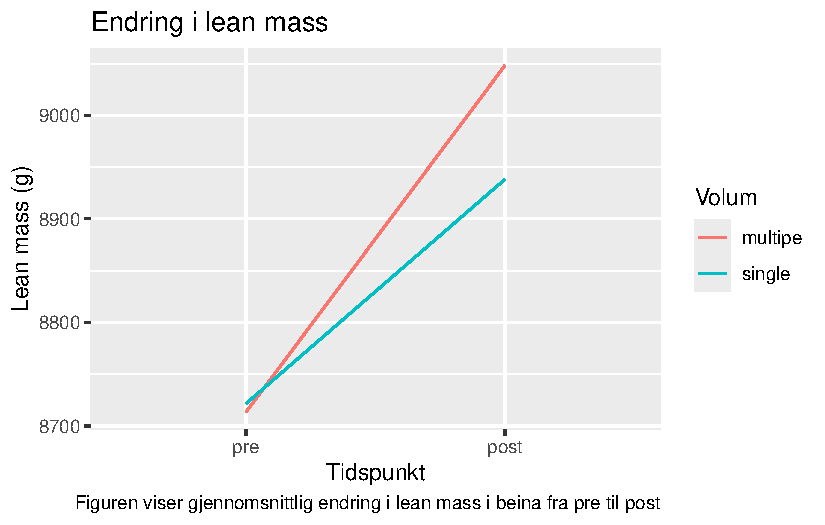
\includegraphics{05-repeated-measurements_files/figure-pdf/unnamed-chunk-3-1.pdf}

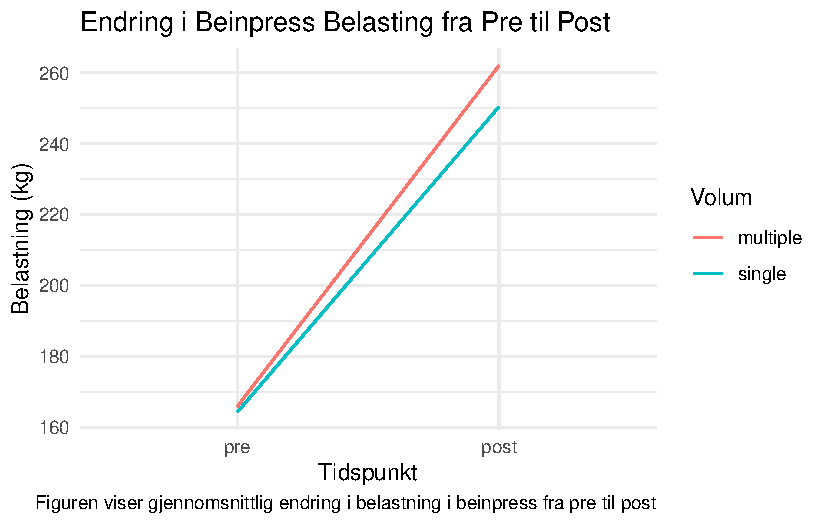
\includegraphics{05-repeated-measurements_files/figure-pdf/unnamed-chunk-5-1.pdf}

\bookmarksetup{startatroot}

\chapter{Diskusjon}\label{diskusjon-4}

Problemstillingen i denne studien var om et versus tre sett hadde størst
økning i muuskelstyrke og muskelmasse.

Resultatene som fremkommer i studien viser at tre sett kontra ett sett
har en signifikant større endring på muskelstyrke og muskelmasse. Basert
på tidligere studier gjort av Kriger i 2009 0g 2010 (Krieger 2009,
2010)hvor en så at styrketrening med moderat volum hadde større effekt
på muskelstyrke og muskelmasse enn med lavt volum. Selvom det vises at å
trene et sett også hadde en stor endring i masse og muskelstyrke.

\bookmarksetup{startatroot}

\chapter{Philosophy of science}\label{philosophy-of-science}

\textbf{Vitenskapsfilosofi oppgave Ifølge Hume er det umulig å rasjonelt
begrunne bruken av induksjon. Hva er argumentet for denne konklusjonen?
Gi en innvending mot ett av premissene i Humes argument og prøv å svare
på denne innvendingen på Humes vegne.}

Hume var en kjent filosof og stilte seg kritisk til bruken av induksjon.
Hume mente at det umulig var rasjonelt å kunne begrunne bruken av
induksjon (Alnes, 2024). Hume sine argumenter for dette var at hvert
induktive argument forutsetter uniformitetsprinsippet.
Uniformitetsprinsippet er antagelsen om at naturen oppfører seg
konsekvent, slik at hendelser som har skjedd tidligere, også vil skje i
fremtiden. Det andre argumentet er at uniformitetsprinsippet ikke har en
rasjonell begrunnelse (Vassend, 2024, Dag1, PPT).

\hfill\break
Hume mente at ikke induksjon kunne brukes rasjonelt. Hume mente at
induksjon blant annet baserte seg på empirisme, at det en erfarte i går
vil kunne predikere at det samme skal skje i morgen. Et eksempel på
dette er at siden sola sto opp i går, vil den også stå opp i morgen. Det
Hume sitt syn stiller seg mest kritisk til er hvordan mangelen på en
rasjonell begrunnelse er med på å anta fremtiden i eksemplet som er gitt
over. Basert på den induktive tankegangen vil man lage sirkulære
argument basert på premisset altså erfaringen man har i dag om at sola
sto opp. Danner et nytt premiss om at sola står opp i morgen og i
fremtiden, og at vi lager en konklusjon på at det vil skje. Med andre
ord, for å rettferdiggjøre vår antagelse om at solen vil stige opp i
morgen, må vi allerede tro på gyldigheten av induksjon, som i sin tur
baserer seg på tidligere erfaringer. Hume sitt poeng er at vi baserer
fremtidige hendelser på fortiden sine hendelser. En innvendig mot Humes
sine premiss er det å kunne predikere fremtiden basert på fortiden.
Mennesker har i tusener av år observert at solen står opp hver dag.
Dette danner en empirisme for at det vil skje i morgen. Som menneske vil
det være vanskelig å skulle drive forskning og leve et hverdagsliv om
man ikke vil predikere fremtiden basert på empiristiske erfaringer.

Humes svar på innvendingen om solens oppgang vil ta for seg ulike
argumenter som belyser begrensningene ved induksjon. For det første vil
han understreke at selv om vi har erfaring med at solen har steget opp
hver dag, gir ikke dette en rasjonell garanti for at den vil fortsette å
gjøre det. Våres erfaringer kan være intuitive, men Hume vil kunne
argumentere for at det er ikke nødvendigvis er en logisk nødvendighet
som binder fremtidens hendelser til hva fortiden viste, og det kan være
en dag solen faktisk ikke står opp. Hume vil videre kunne påpeke
muligheten for feilaktige observasjoner. Historisk har mennesket gjort
mange feil og feil antakelser om naturen, for eksempel trodde en at
jorden var flat og at den ble regnet som sentrum i solsystemet. Dette er
eksempler på at menneskets observasjoner kan være begrensede eller
feiltolkede, noe som gjør det risikabelt å basere forventninger om
fremtiden utelukkende på tidligere erfaringer.

Hume ville også peke på sirkulariteten i argumentasjonen. Når vi bruker
tidligere observasjoner av solen for å rettferdiggjøre fremtidige
forventninger, befinner vi oss i et sirkulært resonnement. Vi vil da
anta at fortiden er relevant for fremtiden, men dette er en induktiv
antagelse som selv krever gyldighet. Samlet sett ville Hume fremheve at
selv om erfaring kan gi en intuitiv følelse av sikkerhet, er det
essensielt å se begrensningene ved induksjon. Erfaring alene kan ikke
garantere nødvendighet, observasjoner kan være feilaktige, og
sirkulariteten i argumentasjonen underminerer påstanden om at vi kan
forutsi fremtidige hendelser basert på fortiden. Dette skaper en dyp
usikkerhet i vår forståelse av kunnskap og hvordan vi anvender induksjon
i vitenskapelig tenkning.

\textbf{Gi en kort beskrivelse av falsifikasjonisme og si litt om
hvorfor Popper var motivert til å utvikle denne teorien. Presenter så
ett problem med teorien og vurder hvorvidt problemet kan løses.}

Falsifikasjonisme er synet, assosiert med Popper, at vitenskapene ikke
bør, eller kan, forsøke å bekrefte hypoteser. Hypotesene kan bare
falsifiseres. For å falsifisere en hypotese trenger man ikke annet enn
deduktive gyldige slutninger ihht Popper. Falsifiserbarhet, som
demarkasjonskriterium for vitenskapelighet, altså kriteriet som skiller
vitenskap fra ikke-vitenskapelige påstander. At en påstand er
falsifiserbar innebærer at det er mulig å vise at den er usann, dersom
den faktisk er usann. Popper var opptatt av hvordan falsifiserbarhet lar
oss skille vitenskap fra pseudovitenskap. Hvis en påstand er
falsifiserbar kan den følgelig karakteriseres som vitenskap. Det har med
bakgrunn i at falsifisering av en hypotese følger deduktiv gyldig
slutning. Bekreftelse innebærer brukt av induksjon som da ikke gir en
sikker slutning. Asymmetri mellom bekreftelse og avkreftelse (Antonsen
et.al, 2023). Vitenskapen gjør ikke fremskritt gjennom å bekrefte
teorier, men gjennom en eliminasjonsprosess der hypoteser som ikke
fungerer blir luket ut. Da får man en gradvis utvikling der teorier som
motsetter seg falsifisering blir stående som dominerende. (inntil man
eventuell får nye og mer overlevelsesdyktige konkurrenter som kommer på
banen) Falsifisering av gale hypoteser gjør at vitenskapen har
fremskritt og vokser. Herding av en hypotese eller teori betyr at den
har blitt utsatt for mange tester og forsøk på falsifisering, men har
overlevd disse uten å bli falsifisert. Dette styrker teoriens
troverdighet og gir den en høy grad av vitenskapelig autoritet. Popper
mente at ingen teori kan sies å være endelig bevist, men en ``herdet''
teori er den beste tilgjengelige vitenskapelige forklaringen på et
fenomen. Et sentralt problem med Karl Poppers syn på vitenskapelig
metode er at hans teori om falsifikasjon ikke fullt ut tar høyde for
kompleksiteten i hvordan hypoteser testes i praksis. Ifølge
Quine-Duhem-teoremet er det umulig å teste en enkelt hypotese isolert,
fordi enhver vitenskapelig test alltid involverer flere hypoteser og
underliggende antakelser (Antonsen et al., 2023). Dette skaper
betydelige utfordringer når det gjelder å avgjøre hvilken hypotese som
faktisk bør forkastes dersom testresultatene ikke stemmer overens med
forventningene.

Når et eksperiment gir avvikende resultater, står forskerne overfor en
krevende beslutning. Siden flere hypoteser er involvert i en gitt test,
kan de i noen tilfeller velge å forkaste observasjonene eller
støttehypotesene i stedet for å utfordre hovedteorien. Dette kan føre
til at teorier opprettholdes til tross for motstridende data, noe som
kan bremse vitenskapelig utvikling. Når slike strategier blir utbredt,
risikerer vitenskapen å stagnere, fordi de nødvendige kritiske
vurderingene og revisjonene av teorier ikke finner sted.

For å håndtere utfordringene knyttet til Quine-Duhem-teoremet og Poppers
falsifikasjonisme, kan flere strategier tas i bruk. For det første bør
forskere anvende den hypotetisk-deduktive metoden, der hypoteser
formuleres med klare og testbare prediksjoner. Dette gjør det mulig å
lage spesifikke forutsigelser som kan måles, noe som igjen gjør det
enklere å identifisere hvilke hypoteser som er ansvarlige for et gitt
resultat. For eksempel kan man i medisinsk forskning formulere en
prediksjon om at en spesifikk behandling vil føre til en målbar
reduksjon i symptomer innen en definert tidsperiode.

Videre bør forskere systematisk teste ad hoc-hypoteser, som ofte
introduseres for å forklare avvik mellom teori og observasjon. Slike
tilleggsforklaringer må undersøkes gjennom målrettede eksperimenter som
eksplisitt tester hvordan de påvirker resultatene. Dette bidrar til å
avdekke om ad hoc-hypotesene faktisk styrker teorien, eller om de
snarere skjuler svakheter som bør revurderes (Antonsen et al., 2023, s.
110--112).

Til slutt bør hypoteser isoleres så langt det lar seg gjøre. Ved å bryte
ned komplekse teorier i mindre komponenter og teste hver del separat kan
forskerne bedre forstå hvilke deler som fungerer, og hvilke som skaper
problemer. Dette hindrer at hele teorien forkastes unødvendig, samtidig
som det sikrer at svakheter i teorien ikke blir ignorert.

Disse strategiene gjør det mulig å håndtere kompleksiteten i
vitenskapelig testing, samtidig som de adresserer svakhetene ved både
Quine-Duhem-teoremet og Poppers falsifikasjonisme. Ved å kombinere
klarere prediksjoner, systematisk testing av tilleggsforklaringer og en
mer isolert tilnærming til hypoteser kan forskerne skape en mer robust
vitenskapelig praksis. Dette bidrar til å sikre fremgang i vitenskapen,
selv når teorier møter motstridende data.

\bookmarksetup{startatroot}

\chapter{RNA ekstraksjon og analyse}\label{rna-ekstraksjon-og-analyse}

\begin{center}\rule{0.5\linewidth}{0.5pt}\end{center}

\begin{center}\rule{0.5\linewidth}{0.5pt}\end{center}

\section{Introduksjon}\label{introduksjon-5}

I forskning finnes flere metoder for å studere genuttrykk, og en av de
mest brukte teknikkene er kvantitativ fluoresens-basert sanntids
polymerase kjedereaksjon (qPCR) (Derveaux, Vandesompele, and Hellemans
2010). Ifølge Kuang et al.~(2018) gir denne metoden en presis
sanntidsmåling av genuttrykk og er særlig verdifull innen
treningsfysiologi for å undersøke hvordan trening påvirker uttrykket av
spesifikke gener. qPCR gjør det mulig å kvantifisere nivåene av et
målgen, for eksempel i muskelvev, og studere hvordan disse nivåene kan
endres som respons på fysiologiske stimuli (Kuang et al. 2018).

Videre beskriver Kuang et al.~(2018) hvordan qPCR kan brukes til å
undersøke treningsinduserte endringer i genuttrykk, inkludert gener
relatert til muskelfibertyper. Dette gir verdifull innsikt i de
molekylære mekanismene bak muskeltilpasning og hvordan gener responderer
på forskjellige faktorer ved trening, noe som bidrar til en dypere
forståelse av treningsinduserte tilpasninger i kroppen (Kuang et al.
2018).

\section{Metode}\label{metode-5}

\subsection{Overordnet metode for kvantifisering av
genuttrykk}\label{overordnet-metode-for-kvantifisering-av-genuttrykk}

Kuang et al.~(2018) skriver så om metoden for å studere genuttrykk.
Første steget er at RNA-et må omdannes til cDNA (komplementært DNA).
Denne prosessen kalles reversert transkripsjon. Videre vil cDNA bli
kopiert slik at man får milliarder av kopier gjennom PCR prosessen.
cDNA-et blir først utsatt for høy temperatur slik at den doble DNA
tråden blir splittet til en enkeltråd (denaturering). Det andre steget
er at temperaturen så senkes. Da vil cDNA-primere kunne binde seg
(annealing). I tredje og siste steget øker temperaturen slik at primere
binder seg og vi får en ny dobbelt tråd (elongering) (Kuang et al.
2018).

Videre beskriver Kuang et al.~(2018) hvordan PCR-syklusen gjentas flere
ganger, og mengden cDNA øker eksponentielt for hver syklus. En vanlig
metode for å overvåke denne prosessen i sanntid er SYBR Green-metoden. I
denne metoden brukes et fluorescerende fargestoff (SYBR Green), som
binder seg til den doble cDNA-tråden. Ved å bruke fluorescens kan man
følge cDNA-amplifikasjonen i sanntid, ettersom det tas et bilde av
fluorscensen etter hver syklus (Kuang et al. 2018).

Fluorescensen øker eksponentielt med hver syklus, ettersom mer cDNA
produseres. Målet med metoden er å identifisere syklisk terskel
(CT)-verdien, som er den syklusen hvor fluorescensen når en
forhåndsbestemt terskelverdi. CT-verdien gir et mål for hvor raskt
fluorescensen når denne terskelen, og dermed hvor mye cDNA som er til
stede i prøven (Kuang et al. 2018). Jo lavere CT-verdi, desto høyere
nivå av det spesifikke målgenet er til stede i prøven. Derfor kan
CT-verdien brukes til å kvantifisere mengden av det målte genet i
forhold til et referansegen eller kontroll (Livak and Schmittgen 2001).

\subsection{Detaljert fremgangsmåte for
qPCR}\label{detaljert-fremgangsmuxe5te-for-qpcr}

Ved start på forsøket ble ferdig cDNA utdelt fra et tidligere
gjennomført styrkeprosjekt av labansvarlig. For å kunne kjøre en qPCR
ble det brukt cDNA og en Master mix. Denne Master mixen bestod av 50 µl
SYBR-green, 20 µl H\textsubscript{2}O og 10 µl primer mix (myhc I, myhc
IIx eller myhc IIa). Det ble i tillegg laget en Master mix som kontroll.
Denne mestod av 50 µl b2m primer mix, 100 µl H\textsubscript{2}O og 250
µl SYBR-green.

\begingroup
\fontsize{12.0pt}{14.4pt}\selectfont

\begin{longtable}{rrr}

\caption{\label{tbl-fortynn}Fortynningsrekkene som ble laget i forsøket}

\tabularnewline

\toprule
Fortynning & Prøve & H2O \\ 
\midrule\addlinespace[2.5pt]
1 & 30 & 0 \\ 
1/10 & 2 & 18 \\ 
1/100 & 2 & 18 \\ 
1/1000 & 2 & 18 \\ 
1/2 & 10 & 10 \\ 
1/20 & 2 & 18 \\ 
1/200 & 2 & 18 \\ 
\bottomrule

\end{longtable}

\endgroup

Forsøket innebar i tillegg å lage to fortynningsrekker (se
Table~\ref{tbl-fortynn}). Der ble det brukt cmyc primer som ble
fortynnet med H\textsubscript{2}O. I 1/1 prøven var det 30 µl ved start.
1/1 prøven ble benyttet i fortynningen av de andre prøvene. Det var til
slutt 20 µl i alle fortynningene.

\begingroup
\fontsize{12.0pt}{14.4pt}\selectfont
\setlength{\LTpost}{0mm}

\begin{longtable}{llllllll}

\caption{\label{tbl-fortynning}Tabelloversikt over fortynningsrekkene i
triplikat}

\tabularnewline

\toprule
 & 5 & 6 & 7 & 8 & 9 & 10 & 11 \\ 
\midrule\addlinespace[2.5pt]
A & cmyc1 & cmyc 2a & cmyc 3a & cmyc 4a & cmyc 2b & cmyc 3b & cmyc 4b \\ 
B & cmyc1 & cmyc 2a & cmyc 3a & cmyc 4a & cmyc 2b & cmyc 3b & cmyc 4b \\ 
C & cmyc1 & cmyc 2a & cmyc 3a & cmyc 4a & cmyc 2b & cmyc 3b & cmyc 4b \\ 
\bottomrule

\end{longtable}

\begin{minipage}{\linewidth}
Slik ble triplikatene plassert i brønnene\\
\end{minipage}
\endgroup

\begingroup
\fontsize{12.0pt}{14.4pt}\selectfont
\setlength{\LTpost}{0mm}

\begin{longtable}{lll}

\caption{\label{tbl-gener}Tabelloversikt over genuttrykkenes
brønnplassering}

\tabularnewline

\toprule
 & 1 & 2 \\ 
\midrule\addlinespace[2.5pt]
A & myhc I & myhc I \\ 
B & myhc I & myhc I \\ 
C & myhc I & myhc I \\ 
D & myhc IIa & myhc IIa \\ 
E & myhc IIa & myhc IIa \\ 
F & myhc IIa & myhc IIa \\ 
G & myhc IIx & myhc IIx \\ 
H & myhc IIx & myhc IIx \\ 
I & myhc IIx & myhc IIx \\ 
J & b2m & b2m \\ 
K & b2m & b2m \\ 
L & b2m & b2m \\ 
\bottomrule

\end{longtable}

\begin{minipage}{\linewidth}
Kolonne 1 = prøver ved uke 0, kolonne 2 = prøver ved uke 12\\
\end{minipage}
\endgroup

Videre ble prøvene pippetert over i brønner etter pippeteringskartet i
Table~\ref{tbl-gener}. Brønnene ble fylt med 8 µl primer-spesifikk prøve
samt 2 µl cDNA-løsning eller kontrolløsning. Deretter ble
fortynningsrekkene (Table~\ref{tbl-fortynning}) pippetert over i sine
respektive brønner. Dette ble utført i triplikat for samtlige prøver.

Deretter ble qPCR-prøven kjørt i sanntids PCR (Applied Biosystems 7500
Fast Real-Time PCR Systems, Life Technologies AS) ved bruk av Quant
Studio 5. Prosessen bestod av tre ulike steg. Første steget var et «Hold
stage», hvor temperaturen økes med 1,99 °C/s opp til 50 °C. Temperaturen
lå deretter konstant på 50 °C i 2 minutter før den videre ble økt med
1,99 °C/s opp til 95 °C, og forble på 95 °C i 2 minutter.

Det neste steget var selve PCR-prosessen, kalt «PCR stage», som besto av
40 sykluser. Én syklus inkluderte 1 sekund på 95 °C, deretter senkes
temperaturen med 1,77 °C/s til 60 °C, hvor temperaturen ble holdt
konstant i 30 sekunder. Etter hver syklus ble det tatt et bilde av
fluoresensen.

Siste steget, kalt «Melt stage», begynte med at temperaturen økte med
1,99 °C/s opp til 95 °C. Temperaturen ble holdt konstant i 15 sekunder,
før den gradvis ble senket med 1,77 °C/s til den nådde 60 °C, hvor
temperaturen ble holdt konstant i 1 minutt. Temperaturen ble deretter
økt med 0,15 °C/s opp til 95 °C, og holdt konstant i 15 sekunder.

Når PCR-prosessen var ferdig, ble CT-verdiene hentet ut. Verdiene ble
deretter databehandlet og analysert ved hjelp av Excel, Microsoft Office
og primer effektiviteten ble beregnet.

\section{Resultater}\label{resultater-1}

\begingroup
\fontsize{12.0pt}{14.4pt}\selectfont
\setlength{\LTpost}{0mm}

\begin{longtable}{llrrrr}

\caption{\label{tbl-ctvals}Ct-verdier}

\tabularnewline

\toprule
Prøve & Genuttrykk & CT1 & CT2 & CT3 & CT gj.snitt \\ 
\midrule\addlinespace[2.5pt]
Kontroll & b2m & 23.43 & 24.07 & 23.32 & 23.61 \\ 
U0 & myhc I & 18.30 & 19.22 & 19.76 & 19.10 \\ 
U12 & myhc I & 18.43 & 19.08 & 18.35 & 18.62 \\ 
U0 & myhc IIa & 22.42 & 17.71 & 18.31 & 19.48 \\ 
U12 & myhc IIa & 18.39 & 18.73 & 35.24 & 24.12 \\ 
U0 & myhc IIx & 25.71 & 25.04 & 23.77 & 24.84 \\ 
U12 & myhc IIx & 25.12 & 23.57 & 23.05 & 23.92 \\ 
\bottomrule

\end{longtable}

\begin{minipage}{\linewidth}
CT gj.snitt = gjennomsnitt av CT1, CT2 og CT3\\
\end{minipage}
\endgroup

Endringen i CT-verdier fra uke 0 til uke 12 viser en reduksjon i antall
sykluser for myhc I, mens for myhc IIa og myhc IIx er det observert en
økning i antall sykluser før CT-verdien nås (Table~\ref{tbl-ctvals}).

\begingroup
\fontsize{12.0pt}{14.4pt}\selectfont
\setlength{\LTpost}{0mm}

\begin{longtable}{lrrr}

\caption{\label{tbl-genes}Prosentvis fordeling av genuttrykk}

\tabularnewline

\toprule
Tidspunkt & myhc I & myhc IIa & myhc IIx \\ 
\midrule\addlinespace[2.5pt]
Uke 0 & 56 & 43 & 1 \\ 
Uke 12 & 95 & 2 & 2 \\ 
\bottomrule

\end{longtable}

\begin{minipage}{\linewidth}
Andel genuttrykk (\%) ved uke 0 og uke 12\\
\end{minipage}
\endgroup

Som vist i Table~\ref{tbl-genes}, økte andelen myhc I markant fra før
til etter treningsintervensjonen. Andelen myhc IIx økte også noe, mens
andelen myhc IIa viste en betydelig reduksjon.

Basert på de gjennomsnittlige CT-verdiene og logaritmen av
fortynningene, ble primerens effektivitet beregnet til 153 \%.

\section{Diskusjon}\label{diskusjon-5}

Målet med forsøket var å undersøke endringer i myosintungkjedene etter
en styrketreningsintervesjon på 12 uker for en utrent forsøksperson ved
hjelp av qPCR.

I forsøket ble det undersøkt hvor mange sykluser de ulike
myosintungkjedene trengte for å nå sin sykliske terskelverdi (CT). Færre
sykluser og lavere CT-verdier indikerer større genuttrykk. Våre
resultater viser en endring i antall sykluser som kreves for at
myosintungkjedene skal nå sin CT-verdi. Den prosentvise endringen for
tungkjedenes CT-verdier er betydelig for myhc I og IIa. Genuttrykket for
myhc I økte betydelig, mens uttrykket for myhc IIa og myhc IIx viste
begge en reduksjon, med en større nedgang for myhc IIa sammenlignet med
myhc IIx.

I en tidligere studie av Ellefsen et al.~(2014), hvor en
styrketreningsintervensjon ble gjennomført på utrente individer over 12
uker, ble det observert en økning i myhc IIa, en reduksjon i myhc IIx,
samt stabilitet i myhc I (Ellefsen et al. 2014). I kontrast til dette
viser våre resultater motstridende funn, med både reduksjon i myhc IIa
og myhc IIx, samt en betydelig økning i myhc I.

Andre studier, som Terzis et al.~(2008) og Andersen et al.~(2000), viste
også at utrente personer med overvekt av myhc IIx opplever en reduksjon
i myhc IIx og en økning i myhc IIa ved trening, med minimal endring i
myhc I (Terzis et al. 2008; Andersen and Aagaard 2000). Det er kjent at
genuttrykk ikke kan endres fra myhc I til myhc IIa eller myhc IIx, noe
som gjør det vanskelig å forklare de resultatene vi har fått fra
analysen av myosintungkjeder. Dette reiser spørsmål om hva som kan ha
skjedd under vår analyse og om det er spesifikke faktorer ved vårt
eksperiment som kan ha bidratt til disse avvikene fra tidligere
forskning.

En mulig kilde til usikkerhet kan være pippeteringsferdighetene og
kvaliteten på primere som ble brukt i forsøket. Det er en risiko for at
primere kan ha vært utgått på dato eller at feil primer ble valgt.
Primerens effektivitet burde ligge mellom 90 \% og 110 \%, men i vårt
tilfelle ble effektiviteten målt til 153 \%. Dette kan tyde på at
menneskelige feil kan ha påvirket resultatene.

Videre er det problematisk å trekke entydige konklusjoner basert på kun
én prøve. I tillegg mangler vi forkunnskap om hvilken type
treningsstimuli deltakerne har vært utsatt for, bortsett fra den
informasjonen vi har fått fra labansvarlig.

\section{Konklusjon}\label{konklusjon-1}

Basert på resultatene vi har fått i dette forsøket, kan vi ikke trekke
noen konklusjoner om endringene i myosintungkjedene for denne
forsøkspersonen. De observerte resultatene er ikke i samsvar med det som
er rapportert i tidligere forskning, og derfor kan vi ikke vurdere disse
funnene som representative eller pålitelige.

\bookmarksetup{startatroot}

\chapter*{References}\label{references}
\addcontentsline{toc}{chapter}{References}

\markboth{References}{References}

\phantomsection\label{refs}
\begin{CSLReferences}{1}{0}
\bibitem[\citeproctext]{ref-andersen2000}
Andersen, Jesper L., and Per Aagaard. 2000. {``Myosin Heavy Chain IIX
Overshoot in Human Skeletal Muscle.''} \emph{Muscle \& Nerve} 23 (7):
1095--1104.
\url{https://doi.org/10.1002/1097-4598(200007)23:7\%3C1095::AID-MUS13\%3E3.0.CO;2-O}.

\bibitem[\citeproctext]{ref-Bassett}
Bassett, D R, Jr, and E T Howley. 2000. {``Limiting Factors for Maximum
Oxygen Uptake and Determinants of Endurance Performance.''} \emph{Med.
Sci. Sports Exerc.} 32 (1): 70--84.

\bibitem[\citeproctext]{ref-breil2010f}
Breil, Fabio A., Simone N. Weber, Stefan Koller, Hans Hoppeler, and
Michael Vogt. 2010. {``Block Training Periodization in Alpine Skiing:
Effects of 11-Day HIT on VO2max and Performance.''} \emph{European
Journal of Applied Physiology} 109 (6): 1077--86.
\url{https://doi.org/10.1007/s00421-010-1455-1}.

\bibitem[\citeproctext]{ref-derveaux2010}
Derveaux, Stefaan, Jo Vandesompele, and Jan Hellemans. 2010. {``How to
Do Successful Gene Expression Analysis Using Real-Time PCR.''}
\emph{Methods} 50 (4): 227--30.
\url{https://doi.org/10.1016/j.ymeth.2009.11.001}.

\bibitem[\citeproctext]{ref-deschenes2004}
Deschenes, Michael R. 2004. {``Effects of Aging on Muscle Fibre Type and
Size:''} \emph{Sports Medicine} 34 (12): 809--24.
\url{https://doi.org/10.2165/00007256-200434120-00002}.

\bibitem[\citeproctext]{ref-ellefsen2014}
Ellefsen, S., O. Vikmoen, E. Zacharoff, I. Rauk, G. Slettaløkken, D.
Hammarström, T. A. Strand, et al. 2014. {``Reliable Determination of
Training{-}Induced Alterations in Muscle Fiber Composition in Human
Skeletal Muscle Using Quantitative Polymerase Chain Reaction.''}
\emph{Scandinavian Journal of Medicine \& Science in Sports} 24 (5).
\url{https://doi.org/10.1111/sms.12185}.

\bibitem[\citeproctext]{ref-Halperin}
Halperin, Israel, David B Pyne, and David T Martin. 2015. {``Threats to
Internal Validity in Exercise Science: A Review of Overlooked
Confounding Variables.''} \emph{Int. J. Sports Physiol. Perform.} 10
(7): 823--29.

\bibitem[\citeproctext]{ref-RN130}
Hopkins, W. G. 2000. {``Measures of Reliability in Sports Medicine and
Science.''} Journal Article. \emph{Sports Med} 30 (1): 1--15.
\url{http://www.ncbi.nlm.nih.gov/pubmed/10907753}.

\bibitem[\citeproctext]{ref-hopkins2009}
Hopkins, William G., Stephen W. Marshall, Alan M. Batterham, and Juri
Hanin. 2009. {``Progressive Statistics for Studies in Sports Medicine
and Exercise Science.''} \emph{Medicine \& Science in Sports \&
Exercise} 41 (1): 3--12.
\url{https://doi.org/10.1249/MSS.0b013e31818cb278}.

\bibitem[\citeproctext]{ref-janssen2000}
Janssen, Ian, Steven B. Heymsfield, ZiMian Wang, and Robert Ross. 2000.
{``Skeletal Muscle Mass and Distribution in 468 Men and Women Aged
18{\textendash}88 Yr.''} \emph{Journal of Applied Physiology} 89 (1):
81--88. \url{https://doi.org/10.1152/jappl.2000.89.1.81}.

\bibitem[\citeproctext]{ref-Joyner}
Joyner, Michael J, and Edward F Coyle. 2008. {``Endurance Exercise
Performance: The Physiology of Champions.''} \emph{J. Physiol.} 586 (1):
35--44.

\bibitem[\citeproctext]{ref-krieger2009}
Krieger, James W. 2009. {``Single Versus Multiple Sets of Resistance
Exercise: A Meta-Regression.''} \emph{Journal of Strength and
Conditioning Research} 23 (6): 1890--1901.
\url{https://doi.org/10.1519/JSC.0b013e3181b370be}.

\bibitem[\citeproctext]{ref-krieger2010}
---------. 2010. {``Single Vs. Multiple Sets of Resistance Exercise for
Muscle Hypertrophy: A Meta-Analysis.''} \emph{Journal of Strength and
Conditioning Research} 24 (4): 1150--59.
\url{https://doi.org/10.1519/JSC.0b013e3181d4d436}.

\bibitem[\citeproctext]{ref-kuang2018}
Kuang, Jujiao, Xu Yan, Amanda J. Genders, Cesare Granata, and David J.
Bishop. 2018. {``An Overview of Technical Considerations When Using
Quantitative Real-Time PCR Analysis of Gene Expression in Human Exercise
Research.''} Edited by Ruslan Kalendar. \emph{PLOS ONE} 13 (5):
e0196438. \url{https://doi.org/10.1371/journal.pone.0196438}.

\bibitem[\citeproctext]{ref-livak2001}
Livak, Kenneth J., and Thomas D. Schmittgen. 2001. {``Analysis of
Relative Gene Expression Data Using Real-Time Quantitative PCR and the
2{-}ΔΔCT Method.''} \emph{Methods} 25 (4): 402--8.
\url{https://doi.org/10.1006/meth.2001.1262}.

\bibitem[\citeproctext]{ref-rhea2002}
Rhea, Matthew R., Brent A. Alvar, Stephen D. Ball, and Lee N. Burkett.
2002. {``Three Sets of Weight Training Superior to 1 Set With Equal
Intensity for Eliciting Strength.''} \emph{The Journal of Strength and
Conditioning Research} 16 (4): 525.
\url{https://doi.org/10.1519/1533-4287(2002)016\%3C0525:TSOWTS\%3E2.0.CO;2}.

\bibitem[\citeproctext]{ref-ruxf8nnestad2014}
Rønnestad, B. R., S. Ellefsen, H. Nygaard, E. E. Zacharoff, O. Vikmoen,
J. Hansen, and J. Hallén. 2014. {``Effects of 12 Weeks of Block
Periodization on Performance and Performance Indices in Well{-}Trained
Cyclists.''} \emph{Scandinavian Journal of Medicine \& Science in
Sports} 24 (2): 327--35. \url{https://doi.org/10.1111/sms.12016}.

\bibitem[\citeproctext]{ref-ruxf8nnestad2014f}
Rønnestad, B. R., J. Hansen, and S. Ellefsen. 2014. {``Block
Periodization of High{-}Intensity Aerobic Intervals Provides Superior
Training Effects in Trained Cyclists.''} \emph{Scandinavian Journal of
Medicine \& Science in Sports} 24 (1): 34--42.
\url{https://doi.org/10.1111/j.1600-0838.2012.01485.x}.

\bibitem[\citeproctext]{ref-ruxf8nnestad2016d}
Rønnestad, B. R., J. Hansen, V. Thyli, T. A. Bakken, and Ø. Sandbakk.
2016. {``5{-}Week Block Periodization Increases Aerobic Power in Elite
Cross{-}Country Skiers.''} \emph{Scandinavian Journal of Medicine \&
Science in Sports} 26 (2): 140--46.
\url{https://doi.org/10.1111/sms.12418}.

\bibitem[\citeproctext]{ref-ruxf8nnestad2007}
Rønnestad, Bent R., Wilhelm Egeland, Nils H. Kvamme, Per E. Refsnes,
Fawzi Kadi, and Truls Raastad. 2007. {``DISSIMILAR EFFECTS OF ONE- AND
THREE-SET STRENGTH TRAINING ON STRENGTH AND MUSCLE MASS GAINS IN UPPER
AND LOWER BODY IN UNTRAINED SUBJECTS:''} \emph{Journal of Strength and
Conditioning Research} 21 (1): 157--63.
\url{https://doi.org/10.1519/00124278-200702000-00028}.

\bibitem[\citeproctext]{ref-ruxf8nnestad2019e}
Rønnestad, Bent R., Sjur J. Øfsteng, and Stian Ellefsen. 2019. {``Block
Periodization of Strength and Endurance Training Is Superior to
Traditional Periodization in Ice Hockey Players.''} \emph{Scandinavian
Journal of Medicine \& Science in Sports} 29 (2): 180--88.
\url{https://doi.org/10.1111/sms.13326}.

\bibitem[\citeproctext]{ref-roth2001}
Roth, Stephen M., Fred M. Ivey, Greg F. Martel, Jeff T. Lemmer, Diane E.
Hurlbut, Eliot L. Siegel, E. Jeffrey Metter, et al. 2001. {``Muscle Size
Responses to Strength Training in Young and Older Men and Women.''}
\emph{Journal of the American Geriatrics Society} 49 (11): 1428--33.
\url{https://doi.org/10.1046/j.1532-5415.2001.4911233.x}.

\bibitem[\citeproctext]{ref-Spiegelhalter}
Spiegelhalter, David. 2020. {``Introducing the Art of Statistics: How to
Learn from Data.''} \emph{Numeracy} 13 (1).

\bibitem[\citeproctext]{ref-RN2511}
Tanner, R. K., and C. J. Gore. 2012. \emph{Physiological Tests for Elite
Athletes 2nd Edition}. Book. Human Kinetics.
\url{https://books.google.no/books?id=0OPIiMks58MC}.

\bibitem[\citeproctext]{ref-terzis2008}
Terzis, Gerasimos, Giorgos Georgiadis, Grigoris Stratakos, Ioannis
Vogiatzis, Stavros Kavouras, Panagiota Manta, Henrik Mascher, and Eva
Blomstrand. 2008. {``Resistance exercise-induced increase in muscle mass
correlates with p70S6 kinase phosphorylation in human subjects.''}
\emph{European Journal of Applied Physiology} 102 (2): 145--52.
\url{https://doi.org/10.1007/s00421-007-0564-y}.

\bibitem[\citeproctext]{ref-wernbom2007}
Wernbom, Mathias, Jesper Augustsson, and Roland Thome?? 2007. {``The
Influence of Frequency, Intensity, Volume and Mode of Strength Training
on Whole Muscle Cross-Sectional Area in Humans:''} \emph{Sports
Medicine} 37 (3): 225--64.
\url{https://doi.org/10.2165/00007256-200737030-00004}.

\end{CSLReferences}




\end{document}
